\clearpage
\makeatletter
\efloat@restorefloats
\makeatother


\begin{appendix}
\section{}
\hypertarget{transition-location-effect-unconstrained-mixture-model}{%
\subsection{Transition location effect (unconstrained mixture
model)}\label{transition-location-effect-unconstrained-mixture-model}}

We present the mixture-model posterior estimates for each of the three
parameter values in the three facets of Figure \ref{fig:crossstudypost}.
Similar to the constrained mixture model, we aggregated the posterior
across conditions\footnote{We aggregated across pre-post test for the
  PLanTra dataset as well as genre and topic of the LIFT data set.} and
removed conditions that might conflate comparisons\footnote{We removed
  the masked writing condition in the GUNNEXP2 and CATO, the dyslexic
  group in the CATO data set, and L2 writing in the SPL2 data set.}. The
resulting posterior allows us to examine differences between transition
locations for each data set associated with each of the three
mixture-model parameters.

\begin{figure}

{\centering 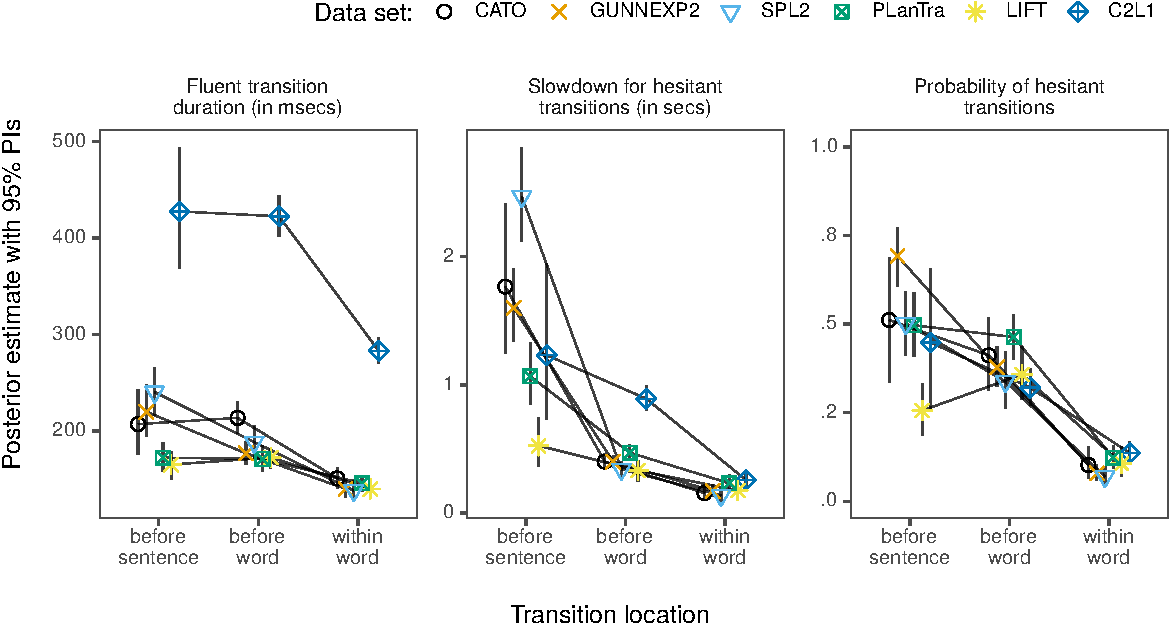
\includegraphics{manuscript_files/figure-latex/crossstudypost-1} 

}

\caption{Mixture model parameter estimates across studies. Distributions of parameter estimates are represented as posterior mean and 95\% probability interval (PI). Estimates for the CATO dataset were calculated for the non-dyslexic group, unmasked condition; also the GUNNEXP2 estimtes represent the unmasked condition; SPL2 estimates are for the L1 group. Axes for transitions durations are log-scaled for visability.}(\#fig:crossstudypost)
\end{figure}

In the following we evaluate differences between transition locations
for all three mixture model parameters. Figure \ref{fig:crossstudypost}
shows largely the same patterns (with caveats) for keystroke interval
estimates by transition location across data sets for all three mixture
model parameters. We found that hesitations appear more frequently at
before-word transitions than within words across data sets (all BFs
\textgreater{} 100). Also hesitations are longer at before-sentence
transitions compared to before-word transitions (all BFs \textgreater{}
100; except for C2L1: BF = 0.35 and LIFT = 2.14) and before-word
transitions compared to within-word transitions (all BF \textgreater{}
10; except for LIFT: BF = 0.71). Further, we observed that fluent
key-transitions are slower at before-word and before-sentence locations
compared to within-word locations (all BFs \textgreater{} 100) but there
is generally no evidence for a difference for fluent transitions for
before-sentence transitions compared to before-word transitions (BFs
\textless{} 0.08; except for SPL2: BF \textgreater{} 100 and GUNNEXP2:
BF \textgreater{} 100). The full results of these pairwise comparisons
can be found in Table \ref{tab:loceffect}.

Hesitation duration tends to be longer at before-sentence locations
compared to before-word locations (except for data sets C2L1 and LIFT)
and longer for before-word locations compared to within-word locations
(except for the LIFT data set). However, for most data set there is
negligible evidence for the idea that writers pause more frequently at
before-sentence locations compared to before-word locations (except for
data sets SPL2 and GUNNEXP2). This is interesting because it is
generally believed that pausing behaviour is associated with syntactic
edges such that more and longer pauses are predicted for key transitions
at larger syntactic edges following the pattern before-sentence \(>\)
before-word \(>\) within-word. In fact, the data set LIFT showed less
pausing before sentences compared to before words. In brief, while
keystroke transitions and pauses tend to be longer and more frequent at
before-word locations compared to within-word transitions, it is not
clear in which contexts keystroke transitions are before-sentence
locations are slower, and their hesitations are longer and more
frequent.

Outstanding is the overall substantially longer fluent transitions for
the C2L1 data. This is presumably reflecting that the population that
this sample is from was the youngest among our data sets presumably
involving the least experienced writers in our data pool. Hesitation
duration and frequencies were similar to the other data sets. There are
some inconsistencies for fluent before-sentence transitions compared to
before-word transitions. Some data sets show before-sentence slowdowns
for fluent transition compared to words. These inconsistencies could, to
some extent, be explained on the basis that data sets differ as to
whether before-sentence transitions involve complex key combination
involve the mean or sum of transitions between space, shift and / or the
sentence-initial letters. In particular, some data include the character
key following the shift key at before sentence location (PLanTra, LIFT)
but others did not scope over the character following the shift key
(CATO, C2L1, SPL2, GUNNEXP2). Notice though that for the data sets
PLanTra and LIFT, there was no evidence for a consistent differences
between before-sentence and before-word transitions (except for longer
hesitations in the PLanTra dataset).

To address this finding, and inconsistency in how before-sentence
transitions were timed, we test to what extent this difference affected
the modelling results for the SPL2 data set. The results are shown in
Appendix \ref{key-combination-effect-unconstrained-mixture-model}. We
found that including the character following the shift key substantially
extends both the transition duration and the hesitation duration but not
the hesitation frequency. However, this conflicts with the absence of
differences in data sets that included the character following shift at
before-sentence transitions (PLanTra, LIFT). In other words, it is
unlikely that patterns in our results can be explained on the basis of
how before-keystroke transitions were operationalised (complex
key-combinations at before-sentence locations).

\blandscape

\begin{center}
\begin{ThreePartTable}

\begin{TableNotes}[para]
\normalsize{\textit{Note.} PI = probability intervals. BF = evidence in favour of the alternative hypothesis over the null hypothesis.}
\end{TableNotes}

\footnotesize{

\begin{longtable}{lrrrrrr}\noalign{\getlongtablewidth\global\LTcapwidth=\longtablewidth}
\caption{\label{tab:loceffect}Effect of transition location on keystroke intervals. Differences are shown on log scale (for transition durations) and logit scale for probability of hesitant transitions. 95\% PIs in brackets.}\\
\toprule
 \multicolumn{1}{c}{ } & \multicolumn{2}{c}{Fluent transitions} & \multicolumn{2}{c}{Hesitation slowdown} & \multicolumn{2}{c}{Hesitation probability} \\
\cmidrule(r){1-1} \cmidrule(r){2-3} \cmidrule(r){4-5} \cmidrule(r){6-7}
Comparison & Est. [95\% PIs] & BF & Est. [95\% PIs] & BF & Est. [95\% PIs] & BF\\
\midrule
\endfirsthead
\caption*{\normalfont{Table \ref{tab:loceffect} continued}}\\
\toprule
 \multicolumn{1}{c}{ } & \multicolumn{2}{c}{Fluent transitions} & \multicolumn{2}{c}{Hesitation slowdown} & \multicolumn{2}{c}{Hesitation probability} \\
\cmidrule(r){1-1} \cmidrule(r){2-3} \cmidrule(r){4-5} \cmidrule(r){6-7}
Comparison & Est. [95\% PIs] & BF & Est. [95\% PIs] & BF & Est. [95\% PIs] & BF\\
\midrule
\endhead
\textbf{C2L1} &  &  &  &  &  & \\
\ \ \ before sentence vs word & 0.01 [-0.13, 0.15] & 0.07 & 0.21 [-0.13, 0.54] & 0.35 & 0.54 [-0.31, 1.43] & 0.89\\
\ \ \ before vs within word & 0.4 [0.38, 0.42] & > 100 & 0.49 [0.39, 0.58] & > 100 & 1.1 [0.76, 1.44] & > 100\\
\textbf{CATO (non-dyslexic, unmasked)} &  &  &  &  &  & \\
\ \ \ before sentence vs word & -0.03 [-0.18, 0.11] & 0.08 & 1.19 [0.88, 1.49] & > 100 & 0.41 [-0.44, 1.27] & 0.67\\
\ \ \ before vs within word & 0.35 [0.31, 0.38] & > 100 & 0.35 [0.14, 0.54] & 17.48 & 1.83 [1.19, 2.49] & > 100\\
\textbf{GUNNEXP2 (unmasked)} &  &  &  &  &  & \\
\ \ \ before sentence vs word & 0.22 [0.12, 0.32] & > 100 & 0.93 [0.78, 1.07] & > 100 & 1.32 [0.86, 1.78] & > 100\\
\ \ \ before vs within word & 0.23 [0.21, 0.25] & > 100 & 0.38 [0.21, 0.54] & > 100 & 1.97 [1.59, 2.37] & > 100\\
\textbf{LIFT} &  &  &  &  &  & \\
\ \ \ before sentence vs word & -0.04 [-0.13, 0.05] & 0.07 & 0.35 [0.05, 0.72] & 2.14 & -0.49 [-1.03, 0] & 1.63\\
\ \ \ before vs within word & 0.21 [0.13, 0.27] & > 100 & 0.26 [-0.16, 0.55] & 0.71 & 1.56 [1.02, 2.16] & > 100\\
\textbf{PLanTra} &  &  &  &  &  & \\
\ \ \ before sentence vs word & 0.01 [-0.09, 0.11] & 0.07 & 0.65 [0.46, 0.83] & > 100 & 0.13 [-0.25, 0.53] & 0.25\\
\ \ \ before vs within word & 0.16 [0.1, 0.21] & > 100 & 0.37 [0.2, 0.54] & > 100 & 1.83 [1.48, 2.17] & > 100\\
\textbf{SPL2 (L1)} &  &  &  &  &  & \\
\ \ \ before sentence vs word & 0.24 [0.17, 0.31] & > 100 & 1.39 [1.25, 1.52] & > 100 & 0.69 [0.17, 1.19] & 8.01\\
\ \ \ before vs within word & 0.31 [0.28, 0.34] & > 100 & 0.35 [0.14, 0.54] & 16.25 & 1.94 [1.4, 2.5] & > 100\\
\bottomrule
\addlinespace
\insertTableNotes
\end{longtable}

}

\end{ThreePartTable}
\end{center}
\elandscape
\end{appendix}
